\chapter{Preface}

\section*{Pulse sequence notation}

Filled black rectangular bars indicate \ang{90} pulses; empty bars indicate \ang{180} pulses.
Pulses with other flip angles are depicted using filled grey bars, typically with the Greek letter $\beta$ above it representing the flip angle.
Delays are variously represented by the letters $\Delta$ and $\tau$, and phases by $\phi$; exact values of these are given in the respective captions.
Decaying sinusoids mark detection periods, sometimes with simultaneous heteronuclear decoupling on other channels (grey boxes labelled `dec.').
$z$-Gradient amplitudes are given as percentages of the maximum gradient amplitude, which is probehead-dependent (see \cref{tbl:spectrometers}).
This maximum amplitude is unlikely to substantially affect the performance of any of the pulse sequences; consequently, I quote gradient amplitudes only as percentages.
In practice, pulse programmes may be implemented with tiny differences in delays to accommodate finite pulse widths and other technicalities.

\section*{Samples used}

The caption of every figure showing experimental data includes a `code' at the end, which indicates the spectrometer and sample used for the data.
These possibilities are enumerated in \cref{tbl:spectrometers,tbl:samples,fig:samples}.
Therefore, for example, the code \texttt{7Z} would represent data acquired on the \SI{700}{\MHz} spectrometer on the zolmitriptan sample.

\begin{table}
    \begin{tabular}{ccl}
        \toprule
        \textbf{Code} & \textbf{Internal name} & \textbf{Details} \\
        \midrule
        \texttt{7} & \href{http://nmrweb.chem.ox.ac.uk/av700.aspx}{AV700} & \makecell[l]{
             \SI{700}{\MHz} \proton{} resonance frequency \\
             \SI{5}{\mm} TCI \proton{}/\carbon{}/\nitrogen{} inverse cryoprobe \\
             \SI{53}{\gauss\per\cm} maximum $z$-gradient amplitude \\
             AVANCE III console, TopSpin 3.6.2
         } \\
         \midrule
        \texttt{6} & \href{http://nmrweb.chem.ox.ac.uk/av600.aspx}{AV600} & \makecell[l]{
             \SI{600}{\MHz} \proton{} resonance frequency \\
             \SI{5}{\mm} Prodigy \ch{N2} broadband cryoprobe (\proton{}/\fluorine{} outer coil) \\
             \SI{66}{\gauss\per\cm} maximum $z$-gradient amplitude \\
             AVANCE III console, TopSpin 3.6.2
         } \\
        \midrule
        \texttt{4} & \href{http://nmrweb.chem.ox.ac.uk/avb400.aspx}{AVB400} & \makecell[l]{
             \SI{400}{\MHz} \proton{} resonance frequency \\
             \SI{5}{\mm} broadband (room-temperature) SmartProbe \\
             \SI{50}{\gauss\per\cm} maximum $z$-gradient amplitude \\
             AVANCE NEO console, TopSpin 4.0.8
         } \\
        \bottomrule
    \end{tabular}
    \caption[Spectrometers used in this thesis]{Spectrometers used in this thesis. A more complete description may be accessed via the links in the `internal name' column.}
    \label{tbl:spectrometers}
\end{table}

\begin{table}
    \begin{tabular}{cccc}
        \toprule
        \textbf{Code} & \textbf{Compound} & \textbf{Solvent} & \textbf{Concentration} \\
        \midrule
        \texttt{A}  & Andrographolide & \dmso      & \SI{40}{\milli\molar}  \\
        \texttt{B}  & (3-Fluorophenyl)boronic acid & \dmso & \SI{120}{\milli\molar}  \\
        \texttt{C}  & Cyclosporin A   & \ch{C6D6}  & \SI{50}{\milli\molar}  \\
        \texttt{E}  & Ethanol         & \ch{D2O}   & \SI{1}{\molar}         \\
        \texttt{F}  & Ferulic acid    & \dmso      & \SI{50}{\milli\molar}  \\
        \texttt{G}  & Gramicidin S    & \dmso      & \SI{40}{\milli\molar}  \\
        \texttt{H}  & Cholesterol     & \ch{CDCl3} & \SI{50}{\milli\molar}  \\
        \texttt{S}  & Sucrose         & 90\% \ch{H2O} / 10\% \ch{D2O} & \SI{22}{\milli\molar}  \\
        \texttt{T}  & Ethyl ferulate  & \dmso      & \SI{200}{\milli\molar} \\
        \texttt{X}  & Brucine         & \ch{CDCl3} & \SI{50}{\milli\molar} \\
        \texttt{Z}  & Zolmitriptan    & \dmso      & \SI{50}{\milli\molar}  \\
        \bottomrule
    \end{tabular}
    \caption[Samples used in this thesis]{Samples used in this thesis. Note that concentrations are approximate and not necessarily constant, as samples were remade over time due to e.g.\ decomposition. However, it is reasonable to assume that the variation in concentration is below 10\%. See \cref{fig:samples} for chemical structures.}
    \label{tbl:samples}
\end{table}

\begin{figure}
    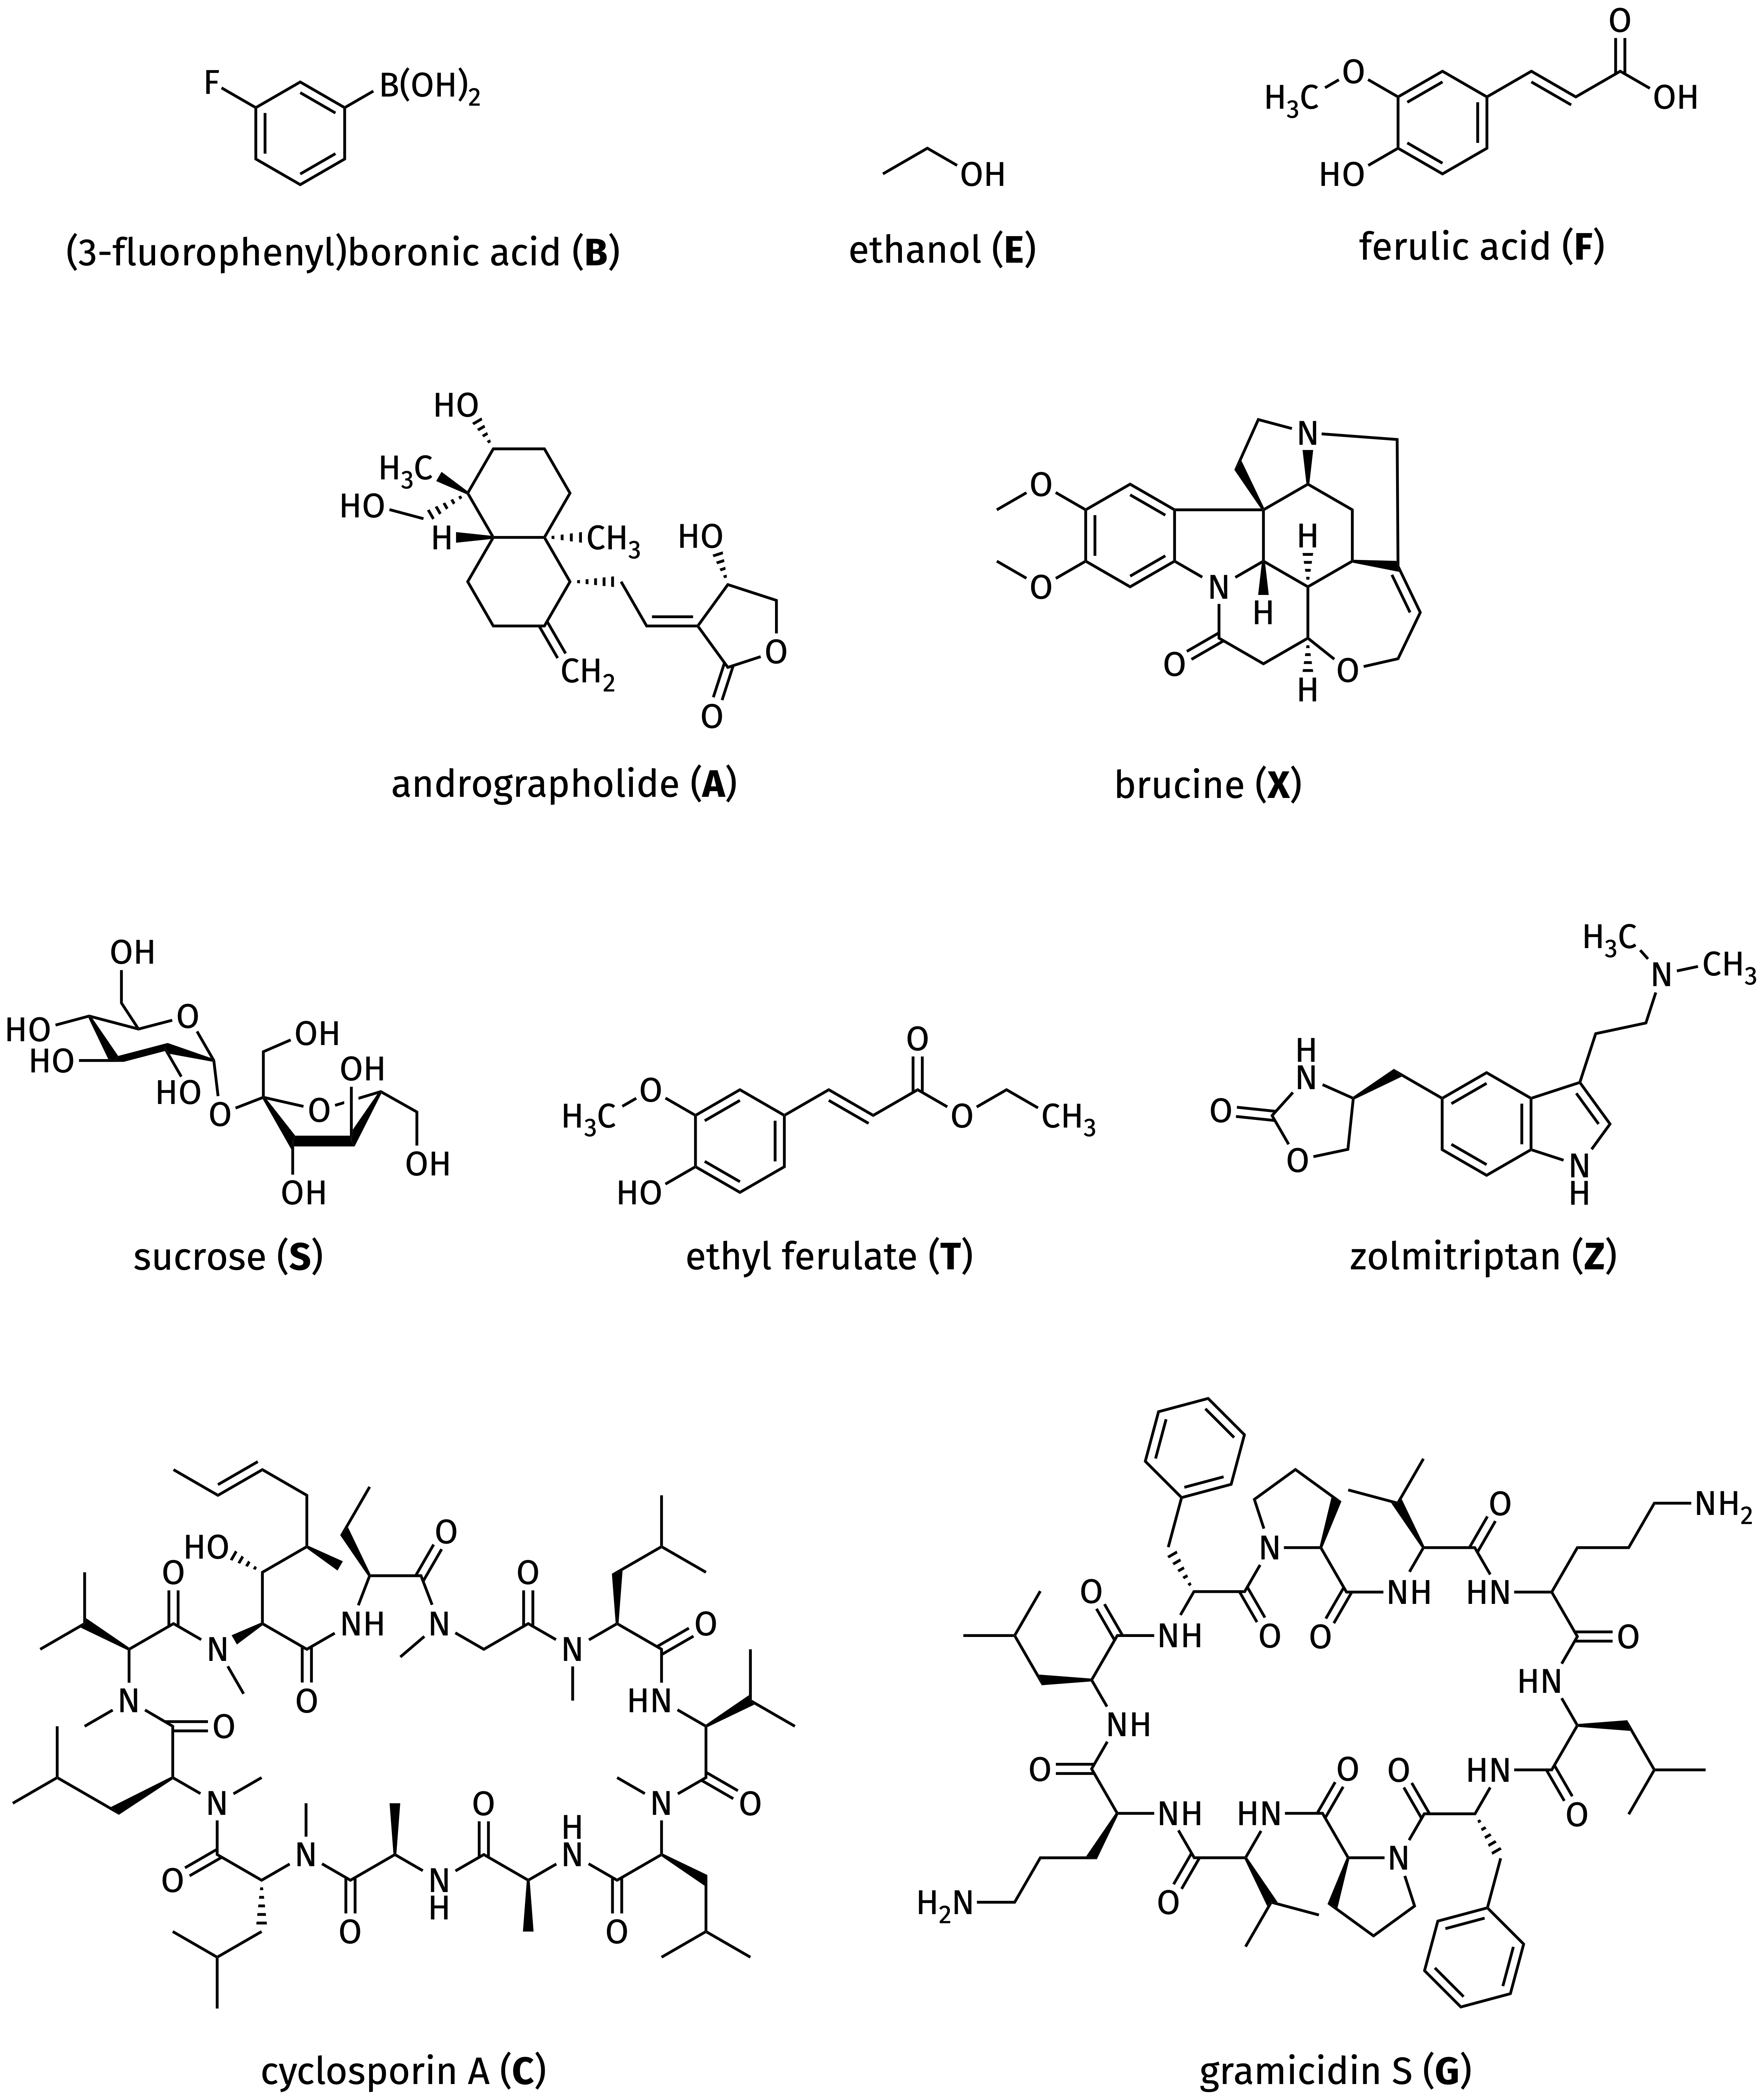
\includegraphics[width=\textwidth]{samples_fira.png}
    \caption[Chemical structures of samples used in this thesis]{Chemical structures of samples used in this thesis. See \cref{tbl:samples} for more information.}
    \label{fig:samples}
\end{figure}

\section*{Software}

All NMR data was processed using TopSpin 3 or 4.
Quantum mechanical NMR simulations were done in Matlab R2021a or R2021b.
This thesis is written using the \LaTeX{} typesetting system: specifically, I used the \LuaLaTeX{} engine.
% The main text font is \href{https://github.com/adobe-fonts/source-serif}{Source Serif 4}, and the mathematics font is \href{https://github.com/alerque/libertinus}{Libertinus Math}.
% The sans-serif font used in figures is Fira Sans, and the monospace font is Fira Code, both part of Mozilla's \href{https://github.com/mozilla/Fira}{Fira family}.
% The $x$-heights don't all match perfectly, but I'm happy enough with it.
% All the fonts are open-source, and can be downloaded from the links provided.

Pulse sequences are drawn using the vector graphics programme \href{https://inkscape.org/}{Inkscape}.
Plots are generated using \href{https://www.python.org/}{Python 3}, using a number of packages (namely: \href{https://github.com/numpy/numpy}{\texttt{numpy}}, \href{https://github.com/scipy/scipy}{\texttt{scipy}}, \href{https://github.com/matplotlib/matplotlib}{\texttt{matplotlib}}, \href{https://github.com/mwaskom/seaborn}{\texttt{seaborn}}, and \href{https://github.com/yongrenjie/penguins}{\texttt{penguins}}, the last of which was written by me, and described further in \cref{sec:appendix/penguins}).
Even if the underlying data was generated in Matlab, I have invariably opted to export it (e.g., to a CSV file) and plot it using Python.

The underlying \LaTeX{} code for this thesis, as well as all figures, can be accessed at TODO (likely GitHub).
